                  
% !Mode:: "TeX:UTF-8"

Neste capítulo serão apresentadas os testes para as funcionalidades disponíveis aos operadores após a instalação do sistema e cadastro dos mesmos.

\section{Certificados}

No menu \textit{Certificados} deve ser possível listar todos os certificados emitidos até o momento para a organização na qual o operador está afiliado, estejam eles ativos ou revogados. Acesse o menu \textit{Certificados $>$ Listar}. Aparecerá uma tela como mostra a figura \ref{fig:listarcertop}. Nesta página deve ser possível ver a data em que foi emitido e a data em que irá expirar cada certificado, bem como o estado em que se encontra (Ativo ou revogado).
É possível realizar as seguintes ações:

\begin{itemize}

	\item \textbf{Download do certificado(}\begin{wrapfigure} 
\includegraphics[height=10]{images/iconedownload} \end{wrapfigure} \textbf{):} Ao clicar nesse ícone você faz o download do certificado selecionado.
	\item \textbf{Revogar certificado(}\begin{wrapfigure} 
\includegraphics[height=10]{images/iconedelete2} \end{wrapfigure} \textbf{):} Quando um certificado estiver ativo, este ícone irá aparecer na linha do respectivo certificado para que este possa ser revogado individualmente. Se houver necessidade de revogar mais certificados, é possível selecioná-los e revogalos de uma só vez através do ícone de revogação no canto inferior direito da imagem. 
	
\end{itemize}

\begin{figure}[ht]
     \centering
     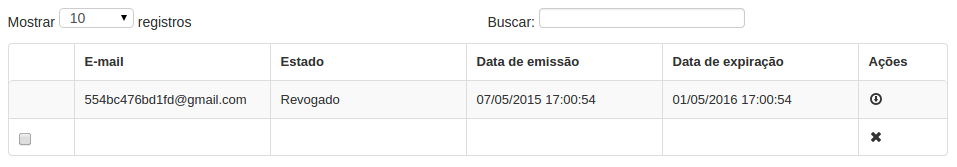
\includegraphics[scale=0.5]{images/listarcertop.png}
     \caption{Listagem de certificados}
     \label{fig:listarcertop}
\end{figure}

\subsubsection{Entradas}
\begin{itemize}

	\item Fazer download de cada um dos certificados 
	\item Revogar um certificado informando a senha de usuário inválida
	\item Revogar um certificado informando a senha de usuário válida
	\item Submeter o formulário para revogação em branco (sem informar o motivo da revogação)
	\item Utilizar a revogação em lotes, clicando no quadrado no canto inferior esquerdo da tabela, utilizando as mesmas entradas citadas acima
	\item Executar busca de certificado através do e-mail, fornecendo um e-mail inválido
	\item Executar busca de certificado através do e-mail, fornecendo um e-mail válido
	
\end{itemize}

\subsubsection{Saídas}

\begin{itemize}

	\item O certificado deve ser baixado imediatamente ao clicar na ação de download, podendo este ser visualizado corretamente após baixado
	\item Devem aparecer alertas ao lado de cada campo preenchido de forma inválida ou submetido em branco
	\item Ao tilizar a revogação em lotes, os certificados que já estiverem revogados não devem ser assinalados na tela
	\item A busca com e-mail inválido deve retornar um erro claro e preciso que informe ao usuário que o certificado não foi encontrado
	\item A busca com e-mail válido deve retornar os certificados emitidos para aquele e-mail
	
\end{itemize}

\subsubsection{Dependência de casos de teste}
Depende se há ou não certificados emitidos. Para este caso de teste, é necessário que o usuário emita pelo menos dois certificados para a instituição na qual o operador é afiliado, seguindo os casos de teste no capítulo de Usuário Final.

\section{Estatísticas}

Esta parte do sistema destina-se à mostrar as estatísticas dos certificados emitidos. “Deve ser possível verificar quantos certificados foram emitidos, quantos estão ativos, quantos estão revogados e quantos estão expirados.

\subsection{Total}

Acesse o menu \textit{Estatísticas $>$ Total}. Aparecerá uma tela como mostra a figura \ref{fig:estotal}. Deve ser possível ver quantos certificados já foram emitidos no total, bem como quantos ainda estão ativos e quantos já foram revogados, mas somente para a instituição na qual o operador é afiliado. Logo em baixo deve ser possível clicar nas organizações e ver as estatísticas em separado de cada uma delas. Como se trata de uma funcionalidade que não requere entradas e saídas, não é necessário um plano de testes.

\begin{figure}[ht]
     \centering
     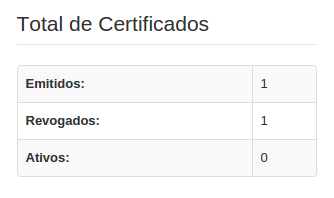
\includegraphics[scale=0.6]{images/estatisticaop.png}
     \caption{Estatísticas total}
     \label{fig:estotalop}
\end{figure}

\subsubsection{Dependência de casos de teste}
Depende se há ou não certificados emitidos. Para este caso de teste, é necessário que o usuário emita pelo menos dois certificados para a instituição na qual o operador é afiliado, seguindo os casos de teste no capítulo de Usuário Final.

\subsection{Procurar por tempo}

Acesse o menu \textit{Estatísticas $>$ Procurar por tempo}. Aparecerá uma tela como mostra a figura \ref{fig:estempo}.

\begin{figure}[ht]
     \centering
     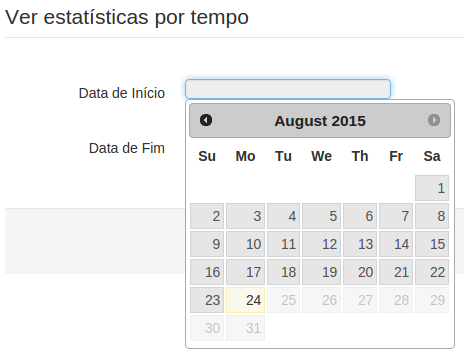
\includegraphics[scale=0.5]{images/estatisticatempo.png}
     \caption{Estatísticas por tempo}
     \label{fig:estempo}
\end{figure}

\subsubsection{Entradas}

\begin{itemize}

    \item Submeter com os campos em branco
	\item Preencher data de início para uma data posterior à de fim
	\item Preencher campos de data de início e fim com data do futuro
	\item Preencher só o campo de data de início, sem preencher a de fim
	\item Preencher só o campo de data de fim, sem preencher a de início
	\item Preencher tudo corretamente e submeter
	
\end{itemize}

\subsubsection{Saídas}

\begin{itemize}

	\item Devem aparecer alertas ao lado de cada campo preenchido de forma inválida ou submetido em branco
	\item Se os dados estiverem todos preenchidos de forma correta o usuário deve ser redirecionado para a tela de estatísticas
	
\end{itemize}

\subsubsection{Dependência de casos de teste}
Depende se há ou não certificados emitidos. Para este caso de teste, é necessário que o usuário emita pelo menos dois certificados para a instituição na qual o operador é afiliado, seguindo os casos de teste no capítulo de Usuário Final.

\section{Atributos}

Através do menu \textit{Atributos $>$ Mapeador de atributos} o operador deve poder configurar os dados que vêm da federação e que vão pertencer ao certificado, como mostra a figura \ref{fig:atmapop}.

\begin{figure}[ht]
     \centering
     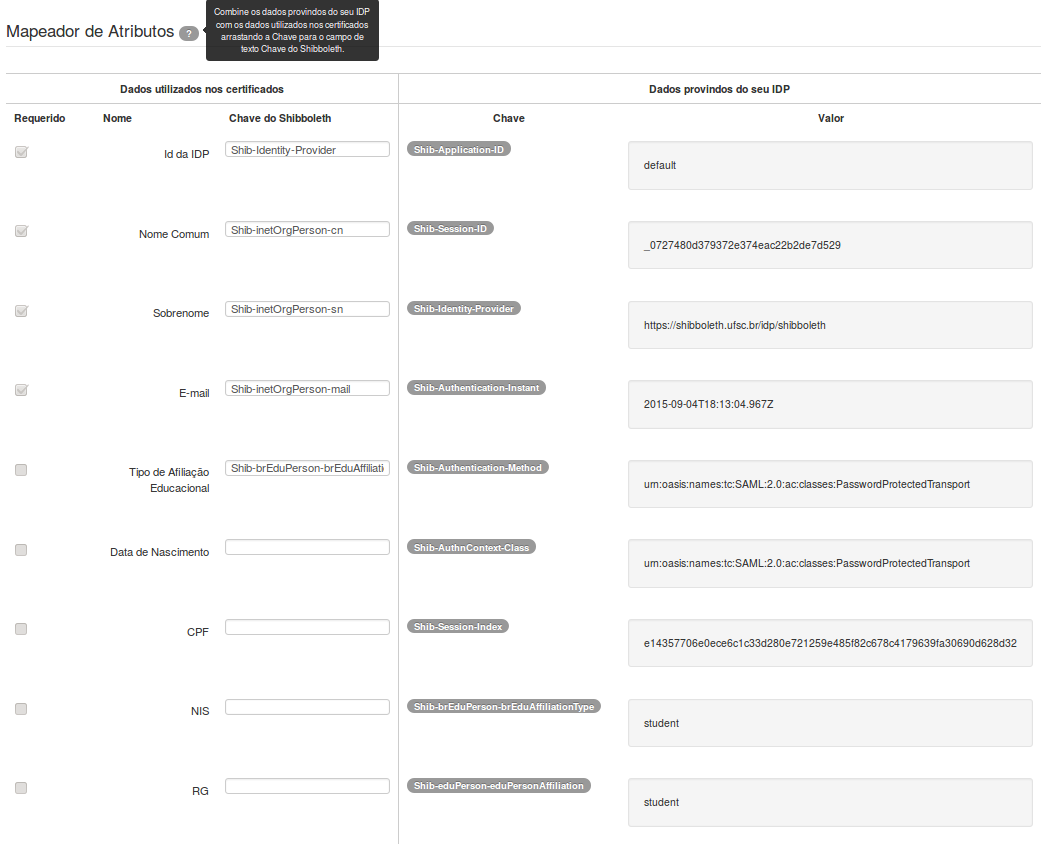
\includegraphics[scale=0.4]{images/oper_attributesmapper.png}
     \caption{Mapeador de atributos}
     \label{fig:atmapop}
\end{figure}

Quando o operador acessar esta tela, os atributos que são necessários configurar já devem vir marcados, pois é o administrador que determina quais atributos vão aparecer no certificado. A tarefa do operador é verificar cada dado que vem da federação e colocá-lo no campo adequado. Por exemplo: Se o CPF for um atributo obrigatório, selecione o CPF na coluna direita, onde estão os dados da federação, e arraste-o para o respectivo campo de CPF na coluna esquerda, onde estão os dados do certificado. É importante deixar claro que é papel do operador conferir se os dados estão configurados com o atributo correto; caso algum atributo esteja com valor incorreto, esta falha não aparecerá nos testes. Por este motivo, não é necessário um caso de teste específico, basta executar a funcionalidade, que deve resultar em "Sucesso" e redirecionar o usuário para a tela inicial.

\section{Alterar dados do usuário e Sair}

O operador deve poder alterar seus dados pessoais e sair do sistema a qualquer momento, basta clicar na engrenagem localizada ao lado superior direito da tela. Duas operações aparecerão: \textit{Alterar dados do usuário} e \textit{Sair}. Ao clicar em \textit{Alterar dados do usuário}, aparecerá uma tela com os campos de dados pessoais, como mostra a figura \ref{fig:alterarop}. Ao clicar em \textit{Sair}, o usuário sai do sistema.

\begin{figure}[ht]
    \centering
     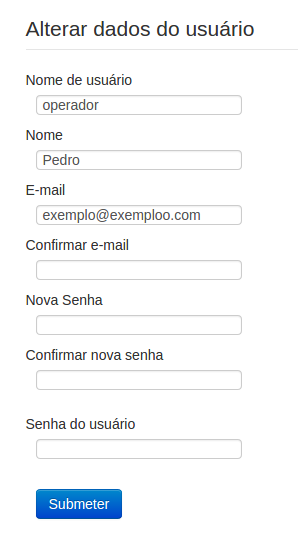
\includegraphics[scale=0.7]{images/alterardadosop.png}
     \caption{Alterar dados do usuário}
     \label{fig:alterarop}
\end{figure}

\subsubsection{Entradas}

\begin{itemize}

	\item Submeter com os campos vazios 
	\item Preencher e-mail sem formatação (ex. operador.com)
	\item Preencher todos os campos, menos confirmação de e-mail e confirmação de nova senha
	\item Preencher confirmação de e-mail e confirmação de senha com entradas diferentes dos campos de e-mail e senha
	\item Submeter formulário com a senha do administrador errada
	\item Submeter o formulário corretamente, com confirmações de e-mail e senha idênticos aos originais, senha de usuário correta, formatação do e-mail válida (operador@teste.com) e nenhum campo em branco
	
\end{itemize}

\subsubsection{Saídas}

\begin{itemize}

	\item Devem aparecer alertas ao lado de cada campo preenchido de forma (formatação) inválida ou submetido em branco
	\item Deve aparecer um alerta de erro se o e-mail e senha de confirmação não forem idênticos aos originais
	\item Deve aparecer um alerta de "senha incorreta" se a senha do usuário estiver errada
	\item Se os dados estiverem todos preenchidos de forma correta, deve aparecer uma mensagem de "Sucesso" e o usuário deve ser redirecionado para a tela inicial
	
\end{itemize}

\subsubsection{Dependência de casos de teste}
Não há dependência com nenhum outro caso de teste.